\section{Overview}\label{sec:overview}

This section presents the design of \tool, a framework for boundary-seeking fuzzing of inter-client state serialization. We first provide an architectural overview of how \tool synthesizes specification knowledge with runtime feedback, following the workflow illustrated in \autoref{fig:overview}. We then formalize the consensus-breaking bug discovery as an optimization problem over the distribution of execution behaviors.

\begin{figure}
    \centering
     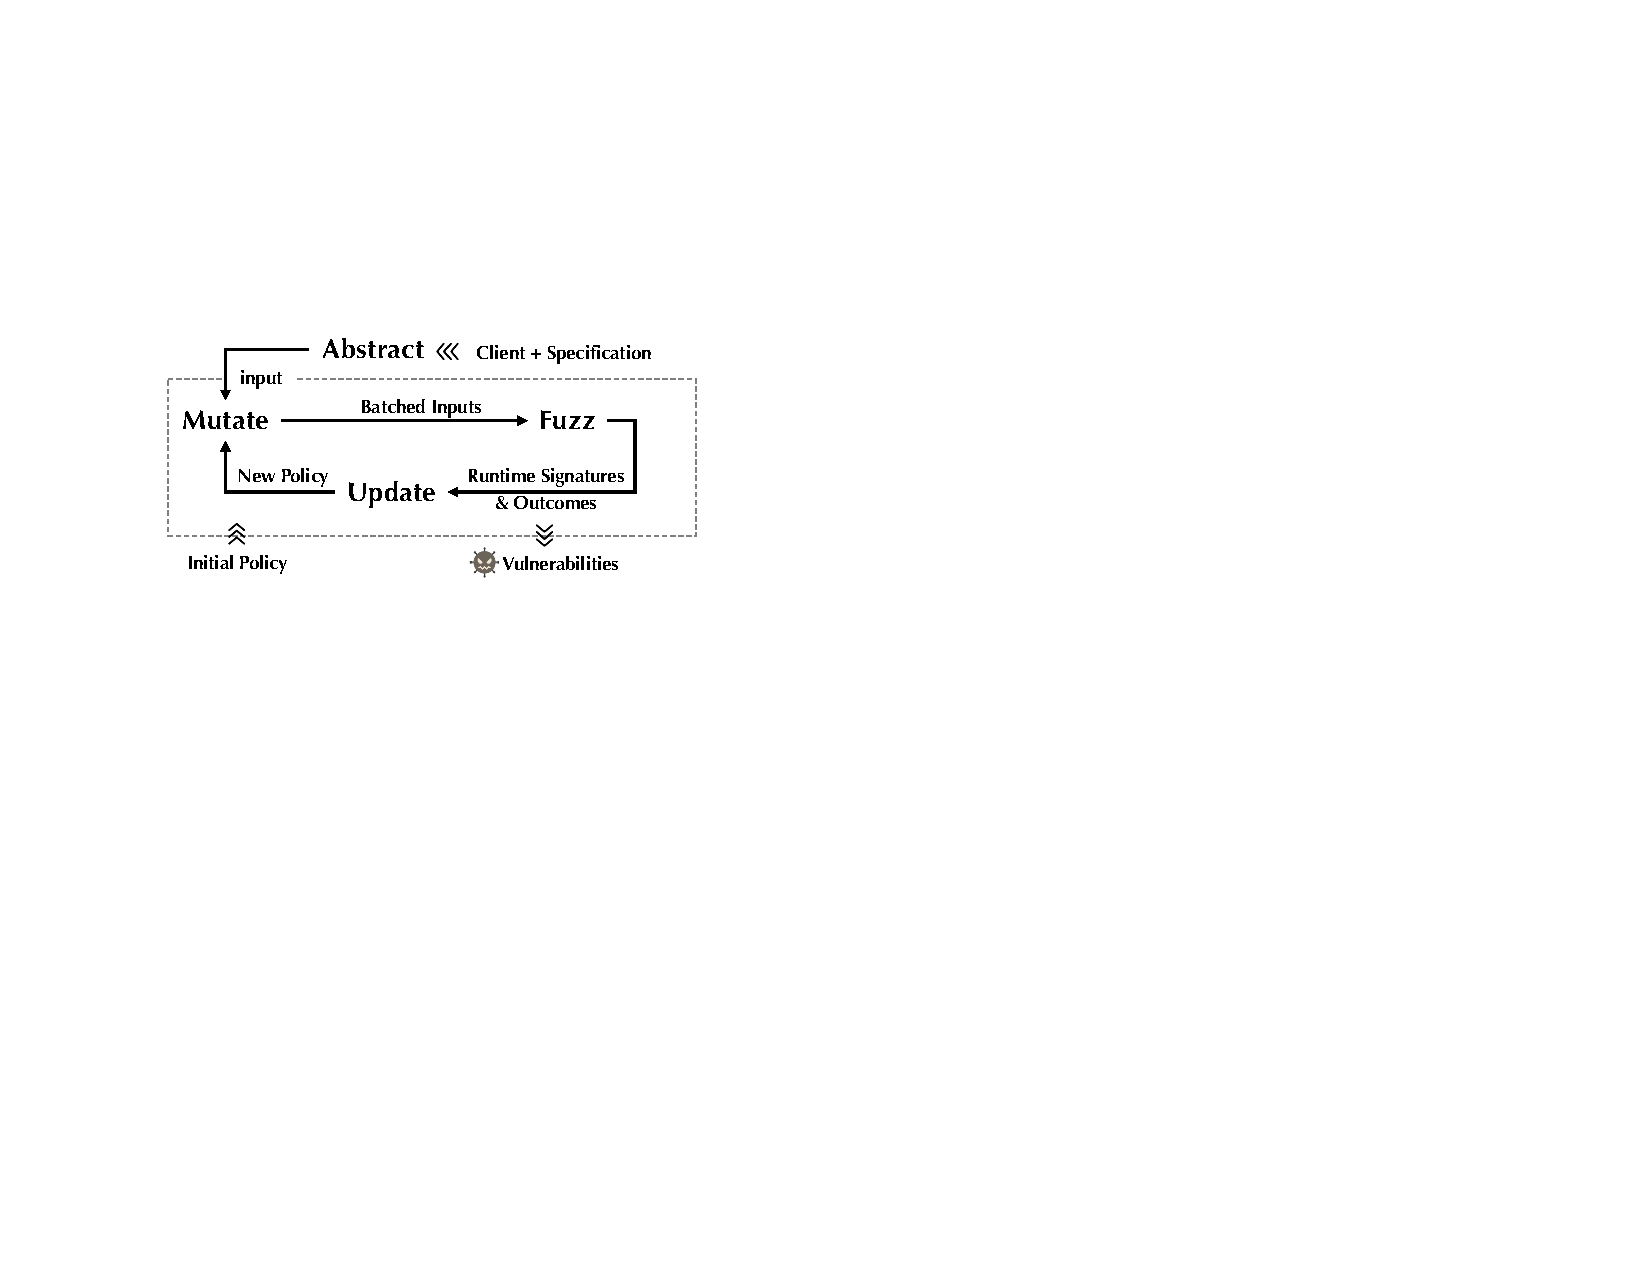
\includegraphics[width=0.95\linewidth]{figs/overview.pdf}
    \caption{An overview of the \tool framework.}
    \label{fig:overview}
\end{figure}

\subsection{Framework Overview}
\begin{figure*}
  \centering
  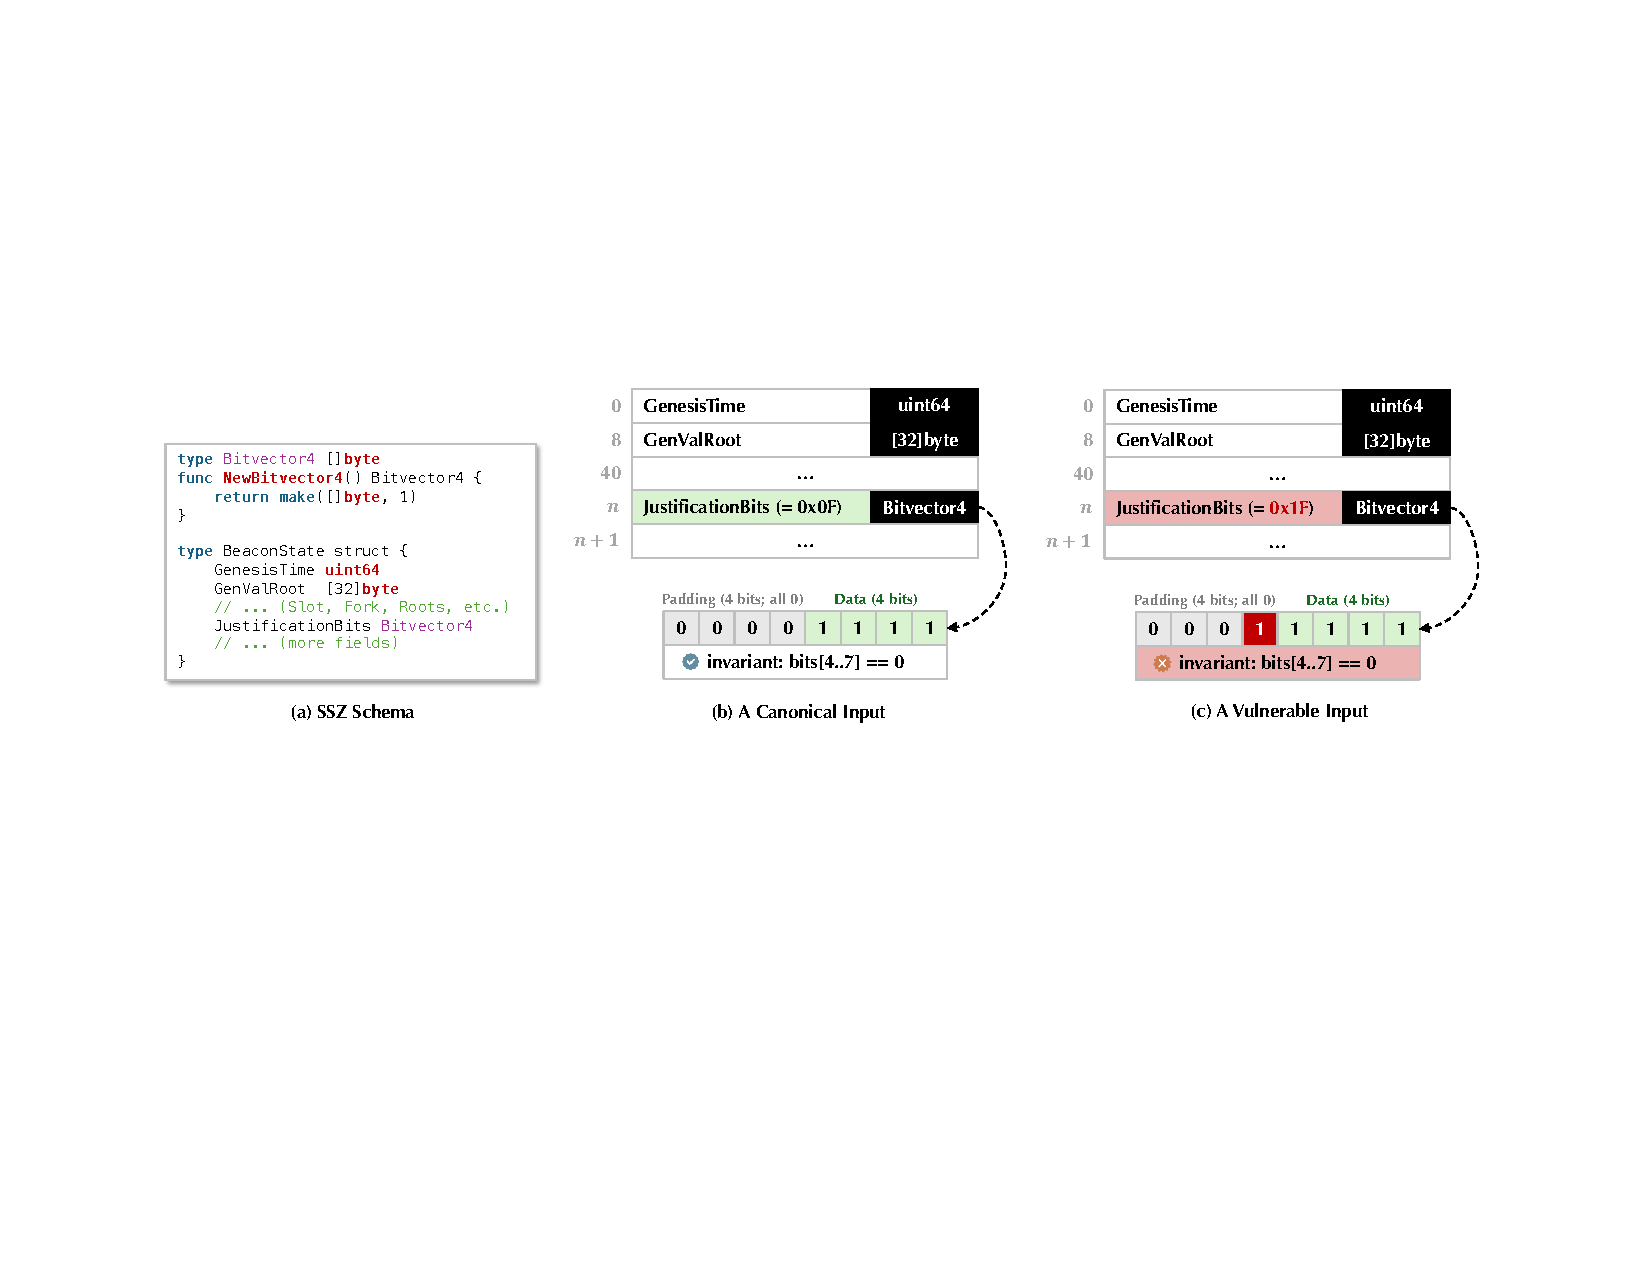
\includegraphics[width=\linewidth]{figs/motivating.pdf}
  \caption{The Bitvector Dirty Padding vulnerability. The SSZ schema (a) defines a \icode{Bitvector4} fitting into one byte. The canonical layout (b) requires zero padding (\icode{0x0F}). A vulnerable layout (c) with a dirty bit (\icode{0x1F}) might be accepted by lenient clients, resulting in a different state root and a consensus split.}
  \label{fig:motivating}
\end{figure*}
As shown in \autoref{fig:overview}, \tool operates as a feedback loop that continuously refines its generation strategy based on execution feedback. The workflow consists of four key components:
\begin{itemize}
    \item \emph{Specification-Guided Abstraction}. Traditional fuzzers operate on raw bytes, often missing semantically critical boundaries defined in the protocol. \tool addresses this by constructing a \emph{specification-guided input abstraction}. By analyzing the client implementation and the protocol specification (e.g., SSZ definitions), \tool derives a set of abstract \emph{buckets} for each field in the data structure. These buckets represent semantic regions of interest, such as canonical values, boundary values (e.g., max length), or non-canonical but semantically valid encodings (e.g., dirty padding). This abstraction transforms the search space from an infinite domain of byte sequences into a structured, finite set of semantic choices.

    \item \emph{Mutate}. Driven by the RL policy, \tool first selects a target abstract bucket (e.g., ``inject dirty padding'') and then instantiates it into a \emph{batch} of concrete inputs. A concretizer generates these inputs by randomizing unconstrained fields while strictly adhering to the boundary constraints of the selected bucket. This step effectively bridges the gap between the high-level semantic strategy and the raw binary data required by the target, ensuring that the generated test cases are concentrated around potentially fragile edge cases.

    \item \emph{Fuzzing (Execution \& Observation)}. The batched inputs are executed against the target consensus client. During execution, \tool uses lightweight instrumentation to capture \emph{runtime signatures}: i.e., a compact representation of the client's internal behavior, including branch coverage, error codes, and validity checks. Unlike traditional fuzzers that only look for crashes, \tool treats the aggregate behaviors of the entire batch as a probability distribution. This distribution captures the \emph{shape} of the client's handling of the current abstract region.

    \item \emph{Update}. The core of \tool's intelligence lies in its update mechanism. The system evaluates the novelty of the current batch by comparing its runtime signature distribution against the history of observed behaviors. We utilize the Kullback-Leibler (KL) divergence to measure this difference~\cite{kullback1951information}. A high divergence indicates that the current policy has successfully steered the client into a new or under-explored behavioral state. This signal serves as a dense reward for the RL agent, updating the policy to favor abstract buckets that continuously push the implementation toward divergent and untested execution paths.
\end{itemize}

\subsection{Motivating Example}

To illustrate why traditional fuzzing falls short in ensuring consensus consistency and how \tool bridges this gap, we consider the ``Bitvector Dirty Padding'' vulnerability. This critical issue was previously found in major Ethereum clients (e.g., Prysm~\cite{prysm}, Teku~\cite{teku}).

\paragraph{The Scenario}
Ethereum's consensus state relies heavily on bitvector types. For example, the \icode{JustificationBits} field is a \icode{Bitvector4}, stored as a single byte where the lower 4 bits represent data and the upper 4 bits are padding. Crucially, the SSZ specification mandates canonicalization, meaning these padding bits \emph{must} be zero.

As visualized in \autoref{fig:motivating}, the canonical encoding for four \icode{true} flags is \icode{0x0F} (binary \icode{0000 1111}). However, a semantically equivalent but \emph{dirty} encoding like \icode{0x1F} (binary \icode{0001 1111}) exists. If a client's decoder fails to enforce the zero-padding check, it will accept \icode{0x1F} as valid. This leads to a consensus split because a strict client rejects the block (invalid hash), while a lenient client accepts it, causing the network to fork.

\paragraph{The Challenge}
Detecting this bug with coverage-guided fuzzing is statistically improbable. A fuzzer mutating raw bytes has a negligible chance of flipping \emph{only} the high-order padding bits while keeping the rest of the structure valid enough to pass initial parsing. Even if it accidentally generates \icode{0x1F}, a vulnerable client will simply accept it without crashing or throwing an error. Without a signal indicating that a dangerous boundary was crossed, the fuzzer treats this as a mundane success and moves on.

\paragraph{\tool's Solution}
\tool addresses this by lifting the exploration from raw bytes to a semantic level, using the specification to define the terrain and RL to navigate it.
\begin{enumerate}
    \item \emph{Mapping the Territory (Specification-Guided Abstraction).} Instead of seeing a flat byte array, \tool analyzes the SSZ specification and identifies \icode{Bitvector[N]} as a type with a specific constraint: ``unused bits must be zero.'' Based on this, it automatically partitions the input space for this field into abstract buckets, such as \irule{Canonical} (padding=0) and \irule{Non-Canonical} (padding$\neq$0). This step explicitly exposes the \emph{dangerous} boundary region that traditional fuzzers miss.

    \item \emph{Sensing the Nuance (RL \& Exploration Reward).} \tool's policy samples from the \irule{Non-Canonical} bucket, and the concretizer generates inputs like \icode{0x1F}. When the client executes this input, it doesn't crash, so there is no obvious bug signal. However, \tool captures the \emph{runtime signatures}, which are trace data showing which checks were performed. Imagine the client usually handles canonical inputs (\icode{0x0F}) via a standard \emph{happy path}. When it handles the dirty input (\icode{0x1F}), even if it accepts it, the internal execution path might subtly shift. For instance, it might skip a specific validation check or iterate differently. \tool compares the distribution of execution behaviors in this new batch against the historical baseline. A high divergence score effectively tells the agent: ``This batch triggered a behavioral profile we haven't seen before; this is surprising and worth exploring further!''

    \item \emph{Closing the Loop (Detection).} Encouraged by this high ``surprise'' reward, the RL policy allocates more budget to this abstract bucket. It generates more variations of dirty padding. Finally, \tool feeds these inputs to a differential oracle (e.g., comparing against a strict reference implementation or checking re-serialization identity). The oracle detects that the input is accepted but hashes differently (or is rejected by the reference), flagging the consensus-breaking vulnerability.
\end{enumerate}

\subsection{Problem Statement}\label{subsec:problem}

We fix a consensus protocol and a serialization schema \(\Gamma\) for some class of consensus states (e.g., blocks or attestations). Let \(\Sigma_\Gamma\) be the set of logical states of shape \(\Gamma\), and let \(\mathcal{B} = \{0,1\}^\ast\) be the set of byte strings. At the level of the protocol specification, the inter-client state serialization for \(\Gamma\) is described by a relation
\[
    \mathcal{R}_\Gamma \subseteq \Sigma_\Gamma \times \mathcal{B},
\]
where \((s,w) \in \mathcal{R}_\Gamma\) means that the byte string \(w\) is an admissible on-the-wire representation of the logical state \(s\). The relation may be non-functional: the spec may single out one canonical encoding for each \(s\), but still allow additional non-canonical yet semantically equivalent encodings. All other \(w \in \mathcal{B}\) are implicitly invalid for \(\Gamma\).

A single client implements this layer by two (possibly partial) functions
\[
    {\sf enc} : \Sigma_\Gamma \to \mathcal{B},
    \quad \mathit{and} \quad
    {\sf dec} : \mathcal{B} \to \Sigma_\Gamma \cup \{\bot\},
\]
where \(\bot\) denotes rejection (parse error, failed validation, and so on). We say that \(({\sf enc},{\sf dec})\) is \emph{serialization-correct} for \(\Gamma\) if it satisfies:
\begin{itemize}
    \item \emph{Decode Soundness}, i.e.:
    \[
        \forall w \in \mathcal{B}.\ {\sf dec}(w) = s \neq \bot \;\Rightarrow\; (s,w) \in \mathcal{R}_\Gamma.
    \]
    \item \emph{Encode-Decode Round-Trip}, i.e.:
    \[
        \forall s \in \Sigma_\Gamma.\ {\sf dec}({\sf enc}(s)) \equiv_{\sf spec} s,
    \]
    where \(\equiv_{\sf spec}\) is the spec’s equality on states of shape \(\Gamma\).
    \item \emph{Decode-Encode Canonicalization}, i.e.: Let \(c : \Sigma_\Gamma \to \mathcal{B}\) be the canonical encoder prescribed by the spec. Then
    \[
        \forall w \in \mathcal{B}.\ {\sf dec}(w) = s \neq \bot \;\Rightarrow\; {\sf enc}(s) = c(s).
    \]
    
\end{itemize}

A \emph{serialization bug} is any \(s \in \Sigma_\Gamma\) or \(w \in \mathcal{B}\) that witnesses a violation of one of the above conditions (unsound acceptance, broken round-trip, or wrong canonicalization). We then formulate the problem we study: For a fixed schema \(\Gamma\) and implementation \(({\sf enc},{\sf dec})\), find byte strings \(w \in \mathcal{B}\) that witness a violation of serialization correctness.
